\documentclass[a3paper,landscape]{article}
\usepackage[left=0cm,top=1in,right=0mm,bottom=0mm]{geometry}
\usepackage{tikz}
\begin{document}
\centering
\begin{tikzpicture}[scale=1]
    \draw (0,0) grid[xstep=\textwidth/27] ({26*(\textwidth/27)},0.875\textheight);
    \foreach \n in {5,...,30}{
    \node[xshift=\textwidth/54] at ({(\n-5)*(\textwidth/27)},-0.5) {\n};
    }    
\end{tikzpicture}
\newpage
\begin{tikzpicture}[scale=1]
    \draw (0,0) grid[xstep=\textwidth/27] ({26*(\textwidth/27)},0.875\textheight);
    \foreach \n in {5,...,30}{
    \node[xshift=\textwidth/54] at ({(\n-5)*(\textwidth/27)},-0.5) {\n};
    }    
    \draw[ultra thick] (0,0) -- ({26*(\textwidth/27)},0) node[midway,yshift=-1.5cm] {\Large Sum of 5 dice};
    \draw[ultra thick] (0,0) -- (0,0.9\textheight) node[sloped,midway,above] {\Large Frequency (Number of times the sum appears)};
\end{tikzpicture}
\newpage
\begin{tikzpicture}[scale=1]
    \draw (0,0) grid[xstep=\textwidth/52] ({51*(\textwidth/52)},0.875\textheight);
    \foreach \n in {10,...,60}{
    \node[xshift=\textwidth/104] at ({(\n-10)*(\textwidth/52)},-0.5) {\n};
    }    
\end{tikzpicture}
\newpage
\begin{tikzpicture}[scale=1]
    \draw (0,0) grid[xstep=\textwidth/52] ({51*(\textwidth/52)},0.875\textheight);
    \foreach \n in {10,...,60}{
    \node[xshift=\textwidth/104] at ({(\n-10)*(\textwidth/52)},-0.5) {\n};
    }    
    \draw[ultra thick] (0,0) -- ({51*(\textwidth/52)},0) node[midway,yshift=-1cm] {\Large Sum of 10 dice};
\end{tikzpicture}
\end{document}